\subsection{\large{\textit{cF}136-Si (Inverse)}}\vspace{-0.1in}
Inverse Clathrate-II


\begin{figure}[H]
\begin{minipage}{0.34\textwidth}\centering
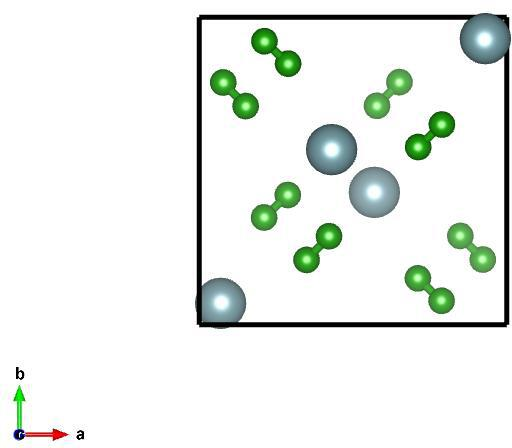
\includegraphics[width=0.9\linewidth,height=2in,keepaspectratio]{/Users/rosecers/work_folders/structures_for_photonics/reference/ref_inp/workspace/392ba9eafabb33baa363ba627992f6a8/final_images/analog_trim.jpg}\\
\small{Image of \textit{cF}136-Si, generated by Vesta}
\end{minipage}\hfill
\begin{minipage}{0.65\textwidth}\raggedright
{\setlength{\mathindent}{0cm}
\begin{equation*}
\begin{split}&\boldsymbol{a_1} = 1/\sqrt{2}\ \hat{y} + 1/\sqrt{2}\ \hat{z}\\[-8pt]
&\boldsymbol{a_2} = 1/\sqrt{2}\ \hat{x} + 1/\sqrt{2}\ \hat{z}\\[-8pt]
&\boldsymbol{a_3} = 1/\sqrt{2}\ \hat{x} + 1/\sqrt{2}\ \hat{y}
\end{split}
\end{equation*}}

\textbf{Space Group:}	227\hspace{0.5in}\textbf{Point Group:}	$m\bar{3}m$\\
\textbf{Inorganic Crystallographic Database} \#56721\\
\textbf{Structure DOI: }\url{10.1103/PhysRevB.60.950}

\end{minipage}\hfill
\end{figure}
\vspace{-0.25in}


\begin{figure}[H]
\begin{minipage}{0.9\textwidth}\centering
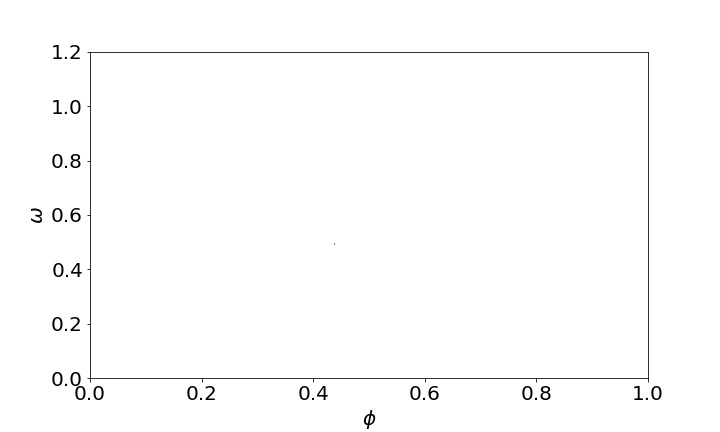
\includegraphics[width=0.9\linewidth,height=2.5in,keepaspectratio]{/Users/rosecers/work_folders/structures_for_photonics/reference/ref_inp/workspace/392ba9eafabb33baa363ba627992f6a8/final_images/gap_atlas.jpg}
\\
\end{minipage}\hfill\caption{Gap Atlas across filling fraction $\phi$ and frequency $\omega$}
\end{figure}


\begin{figure}[H]
\begin{minipage}{0.5\textwidth}\centering
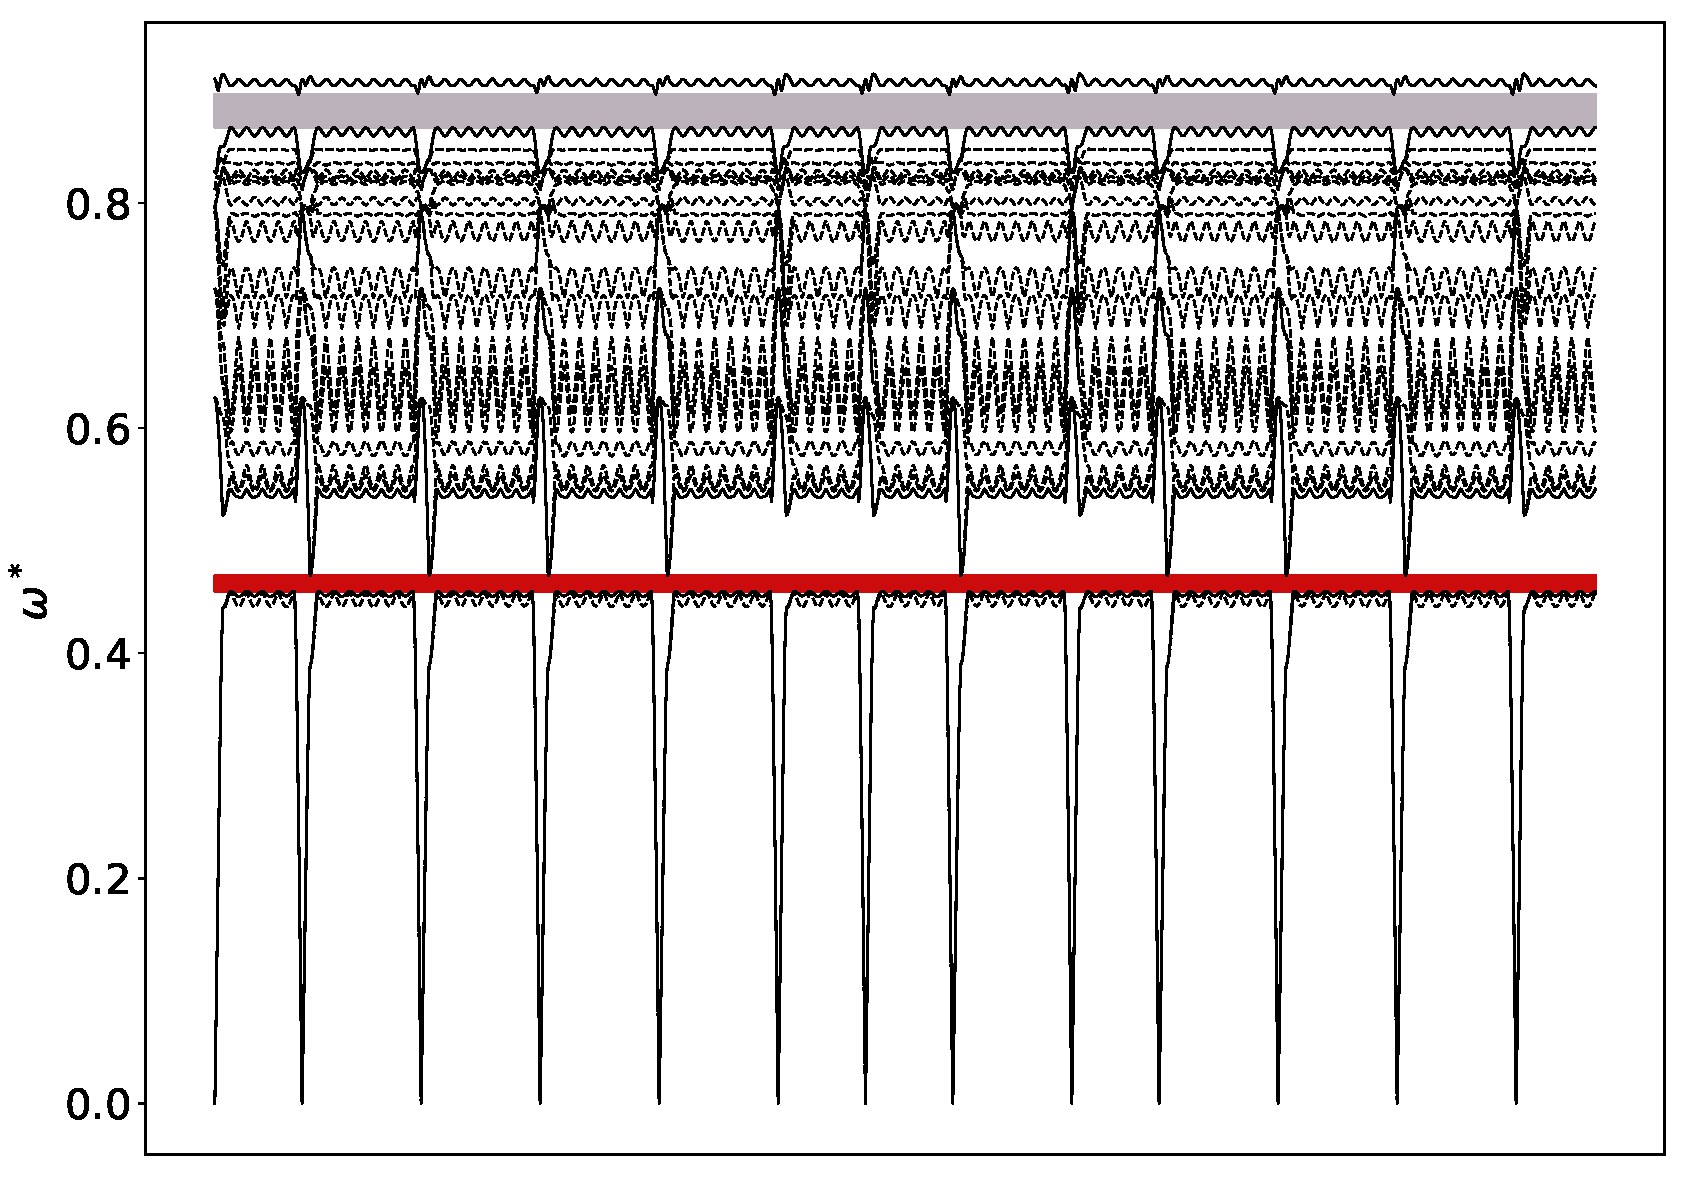
\includegraphics[width=0.9\linewidth,height=1.5in,keepaspectratio]{/Users/rosecers/work_folders/structures_for_photonics/reference/ref_inp/workspace/392ba9eafabb33baa363ba627992f6a8/./final_images/band_diagram_b=2.pdf}
\\Band Structure across 1st BZ
\end{minipage}\hfill
\begin{minipage}{0.48\textwidth}\centering
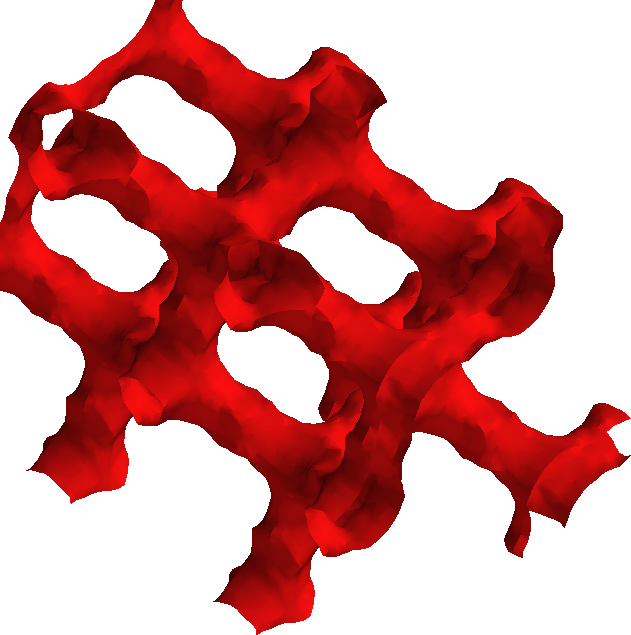
\includegraphics[width=0.9\linewidth,height=1.5in,keepaspectratio]{/Users/rosecers/work_folders/structures_for_photonics/reference/ref_inp/workspace/392ba9eafabb33baa363ba627992f6a8/final_images/cF136-Si_r@gap_2-3.png}
\\View along $a_1$ 
\end{minipage}\hfill\caption{Band Structure and Isosurface of \textit{cF}136-Si (Inverse) at radius = 0.21, filling fraction = 0.153, where the largest gap between bands 2 and 3 occurs with gap size 33.9\%.}

\end{figure}
\vspace{-0.25in}

